\section{Lorentz transformation}
	\setcounter{equation}{0}
	\begin{figure}[h!]
		\centering
		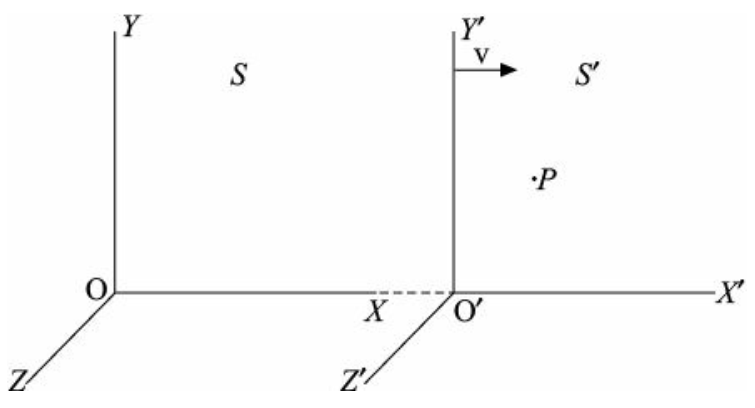
\includegraphics[width=0.55\textwidth]{figures/fig_galilean-transf-01.png}
	\end{figure}
	
	Consider two inertial frames $S$ and $S'$ with coordinate axes $xyz$ and $x'y'z'$ attached to them, with respective origins $O$ and $O'$ respectively. Let the frame $S'$ be moving with respect to $S$ with a uniform velocity $v$ along the $xx'$ axes as shown in the figure above. The origins of the two frames are assumed to coincide when $t=t'=0$.
	
	Because the velocity of $S'$ with respect to $S$ is along the $x$-axis, we have
	\begin{align*}
		y'=y\qq{and}z'=z
	\end{align*}
	
	According to postulate 1, if the motion of a particle is uniformly rectilinear (i.e. in straight line) in frame $S$, then it must be uniformly rectilinear in frame $S'$ as well. Hence the transformation relating $x$ and $x'$ must be linear, thereby written as
	\begin{align}
		x'=\gamma(x-vt) \label{eqn:lorenz-transf:fwd}
	\end{align}
	where $\gamma$ is a dimensionless constant. The inverse transformation is then
	\begin{align}
		x=\gamma(x'+vt') \label{eqn:lorenz-transf:inv}
	\end{align}
	
	Substituting for $x'$ in equation (\ref{eqn:lorenz-transf:inv}) using equation (\ref{eqn:lorenz-transf:fwd}), we have
	\begin{align*}
		x&=\gamma\qty[\gamma(x-vt)+vt'] \\
			&=\gamma^2x-\gamma^2vt+\gamma vt' \\
		\implies \gamma vt'&=\gamma^2vt+x-\gamma^2x \\
			&=\gamma^2vt+(1-\gamma^2)x \\
		\implies t'&=\gamma t+\dfrac{(1-\gamma^2)x}{\gamma v}
	\end{align*}
	Then we can write the tentative transformation equations as
	\begin{equation} \label{eqn:lorentz-transf:tentative}
		\boxed{
			\begin{aligned}
				x'&=\gamma(x-vt) \\
				y'&=y \\
				z'&=z \\
				t'&=\gamma t+\dfrac{(1-\gamma^2)x}{\gamma v}
			\end{aligned}
		}
	\end{equation}
	Let us now consider an EM wave emitted by a point source located at the position $O$ at time $t=0$. The spherical wavefront expands with a speed $c$. Hence the equation of the wavefront in the frame $S$ is
	\begin{align}
		x^2+y^2+z^2&=c^2t^2 \label{eqn:lorentz-transf:sph-wf-01}
	\end{align}
	The corresponding equation in the frame $S'$ is
	\begin{align}
		x'^2+y'^2+z'^2&=c^2t'^2 \label{eqn:lorentz-transf:sph-wf-02}
	\end{align}
	Now, using equations (\ref{eqn:lorentz-transf:tentative}) in equation (\ref{eqn:lorentz-transf:sph-wf-02}), we have
	\begin{align}
		\qty[\gamma(x-vt)]^2+y^2+z^2&=c^2\qty[\gamma t+\dfrac{(1-\gamma^2)x}{\gamma v}]^2 \nonumber\\
		\implies \gamma^2(x-vt)^2+y^2+z^2&=c^2\qty[\gamma^2t^2+\dfrac{(1-\gamma^2)^2x^2}{\gamma^2v^2}+2\gamma t\dfrac{(1-\gamma^2)x}{\gamma v}] \nonumber\\
		\implies \gamma^2x^2+\gamma^2v^2t^2-2\gamma^2xvt+y^2+z^2&=\gamma^2c^2t^2+\dfrac{(1-\gamma^2)^2c^2x^2}{\gamma^2v^2}+2\gamma c^2t\dfrac{(1-\gamma^2)x}{\gamma v} \nonumber\\
		\implies\gamma^2x^2-\dfrac{(1-\gamma^2)^2c^2x^2}{\gamma^2v^2}+y^2+z^2&=\gamma^2c^2t^2-\gamma^2v^2t^2+2\gamma c^2t\dfrac{(1-\gamma^2)x}{\gamma v}+2\gamma^2xvt \nonumber\\
		\implies\qty[\gamma^2-\dfrac{(1-\gamma^2)^2c^2}{\gamma^2v^2}]x^2+y^2+z^2&=\qty[\gamma^2-\gamma^2\dfrac{v^2}{c^2}]c^2t^2+\qty[2c^2\dfrac{(1-\gamma^2)}{v}+2\gamma^2v]xt \label{eqn:lorentz-transf:combn}
	\end{align}
	Comparing with equation (\ref{eqn:lorentz-transf:sph-wf-01}), we find that it has no $xt$ term. Hence the coefficient of the $xt$ term on the RHS of equation (\ref{eqn:lorentz-transf:combn}) must equal zero, i.e.
	\begin{align}
		2c^2\dfrac{(1-\gamma^2)}{v}+2\gamma^2v&=0 \nonumber\\
		\implies\dfrac{2c^2}{v}-\dfrac{2c^2\gamma^2}{v}+2\gamma^2v&=0 \nonumber\\
		\implies\dfrac{2c^2\gamma^2}{v}-2\gamma^2v&=\dfrac{2c^2}{v} \nonumber\\
		\implies\dfrac{2c^2}{v}\gamma^2\qty(1-\dfrac{v^2}{c^2})&=\dfrac{2c^2}{v} \nonumber\\
		\implies\gamma^2\qty(1-\dfrac{v^2}{c^2})&=1 \nonumber\\
		\implies\gamma&=\dfrac{1}{\sqrt{1-v^2/c^2}} \label{eqn:lorentz-transf:gamma}
	\end{align}
	Using equation (\ref{eqn:lorentz-transf:gamma}) in equations (\ref{eqn:lorentz-transf:tentative}), we obtain the expressions for $x'$ and $t'$ as follows:\vspace{-1.5em}
	\begin{multicols}{2}
		%\setlength{\columnseprule}{0.4pt}
		\begin{align*}
			x'&=\gamma(x-vt) \\
			\implies x'&=\dfrac{x-vt}{\sqrt{1-v^2/c^2}}
		\end{align*}		
		%\columnbreak
		
		\begin{align*}
			t'&=\gamma t+\dfrac{(1-\gamma^2)x}{\gamma v} \\
				&=\gamma\qty[t+\dfrac{(1-\gamma^2)x}{\gamma^2v}]=\gamma\qty[t+\qty(\dfrac{1}{\gamma^2}-1)\dfrac{x}{v}] \\
				&=\gamma\qty[t+\qty(1-\dfrac{v^2}{c^2}-1)\dfrac{x}{v}]=\gamma\qty[t-\dfrac{vx}{c^2}] \\
			\implies t'&=\dfrac{t-(vx/c^2)}{\sqrt{1-v^2/c^2}}
		\end{align*}
		
	\end{multicols}
	
	We call $\gamma=\dfrac{1}{\sqrt{1-v^2/c^2}}$ the \emph{relativistic factor} and introduce $\beta=\dfrac{v}{c}$ as the \emph{velocity ratio}, both of which are dimensionless quantities. Then we can write
	\begin{align*}
		\gamma=\dfrac{1}{\sqrt{1-\beta^2}}
	\end{align*}
	
	As per the second postulate, we must always have
	\begin{align*}
		v\leqslant c&\implies\dfrac{v}{c}\leqslant 1 \\
		\implies\beta&\leqslant 1
	\end{align*}
	Then we must also have
	\begin{align*}
		\beta^2&\leqslant 1 \\
		\implies 1-\beta^2&\leqslant 1 \\
		\implies\sqrt{1-\beta^2}&\leqslant 1 \\
		\implies\dfrac{1}{\sqrt{1-\beta^2}}&\geqslant 1 \\
		\implies\gamma&\geqslant 1
	\end{align*}
	Hence, remember $\boxed{\beta\leqslant 1}$ and $\boxed{\gamma\geqslant 1}$.
	
	Now, we have
	\begin{align*}
		x'&=\dfrac{x-vt}{\sqrt{1-v^2/c^2}} \\
			&=\gamma\qty(x-vt) \\
		\implies x'&=\gamma\qty(x-\beta ct)\qq{[$\because$ $v=\beta c$]}
	\end{align*}
	
	Again, we have
	\begin{align*}
		t'&=\dfrac{t-(vx/c^2)}{\sqrt{1-v^2/c^2}} \\
			&=\gamma\qty(t-\dfrac{vx}{c^2}) \\
			&=\gamma\qty(t-\dfrac{\beta cx}{c^2})=\gamma\qty(t-\dfrac{\beta}{c}x) \\
		\implies ct'&=\gamma\qty(ct-\beta x)
	\end{align*}
	Therefore the transformation equations, from $S$ to $S'$, that keep the speed of light constant in both frames are as follows:
	\begin{equation} \label{eqn:lorentz-transformations}
		\boxed{
			\begin{aligned}
				x'&=\gamma\qty(x-\beta ct) \\
				y'&=y \\
				z'&=z \\
				ct'&=\gamma\qty(ct-\beta x)
			\end{aligned}
		}
	\end{equation}
	Equations (\ref{eqn:lorentz-transformations}) are known as the \emph{Lorentz transformation equations}.
	
	For the inverse transformation, from $S'$ to $S$, we need to replace $v$ with $-v$, which implies that $\beta$ would be replaced by $-\beta$. However, the form of the equations remain the same as in equation (\ref{eqn:lorentz-transformations}) because of the first postulate.
	
	Hence the \emph{inverse Lorentz transformation} equations are
	\begin{equation} \label{eqn:lorentz-transformations:inverse}
		\boxed{
			\begin{aligned}
				x&=\gamma\qty(x'+\beta ct') \\
				y&=y' \\
				z&=z' \\
				ct&=\gamma\qty(ct'+\beta x')
			\end{aligned}
		}
	\end{equation}
	
	\subsection{Upper speed limit of the universe}
		Suppose we assume that the relative speed between the frames is larger than the speed of light, i.e. $v>c$, in violation of the first postulate.
		
		Then we would have
		\begin{align*}
			\dfrac{v}{c}>1\implies&\dfrac{v^2}{c^2}>1 \\
			\implies&1-\dfrac{v^2}{c^2}<0 \\
			\implies&\sqrt{1-\dfrac{v^2}{c^2}}\text{ is imaginary} \\
			\implies&\gamma=\dfrac{1}{\sqrt{1-v^2/c^2}}\text{ is also imaginary}
		\end{align*}
		This implies that the space and time coordinates of events in $S$ and $S'$ would also be imaginary. But this is physically impossible.
		
		Hence, our assumption is incorrect, i.e. it is not possible for the relative speed between inertial frames to be greater than the speed of light.
		
		In other words, nothing in our universe can move faster than light!
	
	
	\subsection{Matrix form of the Lorentz transformation}
		We can re-write equation (\ref{eqn:lorentz-transformations}) as follows:
		\begin{align*}
			x'&=\gamma\cdot x+0\cdot y+0\cdot z+(-\beta\gamma)\cdot(ct) \\
			y'&=0\cdot x+1\cdot y+0\cdot z+0\cdot(ct) \\
			z'&=0\cdot x+0\cdot y+1\cdot z+0\cdot(ct) \\
			(ct)'&=(-\beta\gamma)\cdot x+0\cdot y+0\cdot z+\gamma\cdot(ct)
		\end{align*}
		The above equations may now be collected in the form of the following matrix equation:
		\begin{align*}
			\begin{bmatrix}
				{x'} \\
				{y'} \\
				{z'} \\
				{ct'}
			\end{bmatrix}=\begin{bmatrix}
				{\gamma} & {0} & {0} & {-\beta\gamma} \\
				{0} & {1} & {0} & {0} \\
				{0} & {0} & {1} & {0} \\
				{-\beta\gamma} & {0} & {0} & {\gamma}
			\end{bmatrix}\begin{bmatrix}
			{x} \\
			{y} \\
			{z} \\
			{ct}
			\end{bmatrix}
		\end{align*}
		We define the \emph{Lorentz transformation matrix} as
		\begin{align*}
			\vb{L}=\begin{bmatrix}
				{\gamma} & {0} & {0} & {-\beta\gamma} \\
				{0} & {1} & {0} & {0} \\
				{0} & {0} & {1} & {0} \\
				{-\beta\gamma} & {0} & {0} & {\gamma}
			\end{bmatrix}
		\end{align*}
		which allows us to write the \emph{Lorentz transformation in matrix form} as follows:
		\begin{align*}
			\vb{x'}&=\vb{L}\vb{x}
		\end{align*}
		where $\vb{x'}$ and $\vb{x}$ are the following column matrices containing the coordinates:
		\begin{align*}
			\vb{x'}=\begin{bmatrix}
				{x'} \\
				{y'} \\
				{z'} \\
				{ct'}
			\end{bmatrix}\qq{and}\vb{x}=\begin{bmatrix}
					{x} \\
					{y} \\
					{z} \\
					{ct}
				\end{bmatrix}
		\end{align*}
		Likewise, the \emph{inverse Lorentz transformation in matrix} form can be written as
		\begin{align*}
			\vb{x}&=\vb{L}^{-1}\vb{x'}
		\end{align*}
		where the inverse \emph{Lorentz transformation matrix} is
		\begin{align*}
			\vb{L}^{-1}=\begin{bmatrix}
				{\gamma} & {0} & {0} & {\beta\gamma} \\
				{0} & {1} & {0} & {0} \\
				{0} & {0} & {1} & {0} \\
				{\beta\gamma} & {0} & {0} & {\gamma}
			\end{bmatrix}
		\end{align*}